\chapter{中华人民共和国}
\label{cha:china}

\section{图的例子}
\label{sec:other}

在第~\ref{cha:intro} 章中我们学习了贝叶斯公式~(\ref{equ:chap1:bayes}),这里我们复
习一下:
\begin{equation}
\label{equ:chap2:bayes}
p(y|\mathbf{x}) = \frac{p(\mathbf{x},y)}{p(\mathbf{x})}=
\frac{p(\mathbf{x}|y)p(y)}{p(\mathbf{x})}
\end{equation}

\subsection{绘图}
\label{sec:draw}

本模板不再预先装载任何绘图包(如 \textsf{pstricks,pgf} 等),完全由你自己来决定。
个人觉得 \textsf{pgf} 不错,不依赖于 Postscript。此外还有很多针对 \LaTeX{} 的
 GUI 作图工具,如 XFig(jFig), WinFig, Tpx, Ipe, Dia, Inkscape, LaTeXPiX,
jPicEdt, jaxdraw 等等。

\subsection{插图}
\label{sec:graphs}
关于子图形的使用细节请参看 \textsf{subcaption} 的说明文档。

\subsection{一个图形}
\label{sec:onefig}
一般图形都是处在浮动环境中。之所以称为浮动是指最终排版效果图形的位置不一定与源文
件中的位置对应\footnote{This is not a bug, but a feature of
\LaTeX!},这也是刚使 用 \LaTeX{}
同学可能遇到的问题。如果要强制固定浮动图形的位置,请使用
\textsf{float} 宏包, 它提供了 \texttt{[H]}
参数,比如图~\ref{fig:heythere}。
\begin{figure}[H] % use float package if you want it here
  \centering
  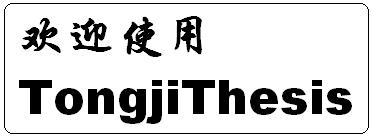
\includegraphics[height=2cm]{hello.jpg}
  \caption{插个图插个图}
  \label{fig:heythere}
\end{figure}

大学之道,在明明德,在亲民,在止于至善。知止而后有定;定而后能静;静而后能安;安
而后能虑;虑而后能得。物有本末,事有终始。知所先后,则近道矣。古之欲明明德于天
下者,先治其国;欲治其国者,先齐其家;欲齐其家者,先修其身;欲修其身者,先正其心;
欲正其心者,先诚其意;欲诚其意者,先致其知;致知在格物。物格而后知至;知至而后
意诚;意诚而后心正;心正而后身 修;身修而后家齐;家齐而后国治;国治而后天下
平。自天子以至于庶人,壹是皆以修身为本。其本乱而未治者 否矣。其所厚者薄,而其所
薄者厚,未之有也!

\hfill \pozhehao《大学》


\subsection{简单子图}
\label{sec:multifig}

如果多个图形相互独立,并不共用一个图形计数器,那么用 \verb|minipage| 或者
\verb|parbox| 就可以。否则,请参看图~\ref{fig:big1},它包含两个小图,分别是图~\ref{fig:subfig1}
和图~\ref{fig:subfig2}。推荐使用 \verb|\subcaption|,不要再用\verb|\subfloat|,\verb|\subfigure| 和 \verb|\subtable|了。
\begin{figure} %[h]
  \centering%
  \subcaptionbox{第一个小图形\label{fig:subfig1}}{%    
    
\includegraphics[height=2cm]{tongji-fig-logo.png}}\hspace{4em}%
  \subcaptionbox{第二个小图形。如果标题很长的话,它会自动换行,这个 caption 就是这样的例子\label{fig:subfig2}}{%    
    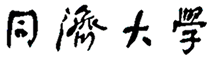
\includegraphics[height=2cm]{tongji-text-logo.png}}
  \caption{包含子图形的大图形}
  \label{fig:big1}
\end{figure}

古之学者必有师。师者,所以传道受业解惑也。人非生而知之者,孰能无惑?惑而不从师,
其为惑也,终不解矣。生乎吾前,其闻道也固先乎吾,吾从而师之;生乎吾後,其闻道也亦
先乎吾,吾从而师之。吾师道也,夫庸知其年之先後生於吾乎!是故无贵无贱无长无少,道
之所存,师之所存也。

嗟乎!师道之不传也久矣,欲人之无惑也难矣。古之圣人,其出人也远矣,犹且从师而问焉;
今之众人,其下圣人也亦远矣,而耻学於师。是故圣益圣,愚益愚。圣人之所以为圣,愚
人之所以为愚,其皆出於此乎?爱其子,择师而教之,於其身也,则耻师焉,惑焉。彼童子
之师,授之书而习其句读者,非吾所谓传其道、解其惑者也。句读之不知,惑之不解,或师
焉,或不焉,小学而大遗,吾未见其明也。巫医、乐师、百工之人不耻相师,  士大夫之族
曰“师”曰“弟子”之云者,则群聚而笑之。问之,则曰:彼与彼年相若也,道相似也,位
卑则足羞,官盛则近谀。呜呼!师道之不复,可知矣。巫医、乐师、百工之人。吾子不齿,
今其智乃反不能及,其可怪也欤!圣人无常师。孔子师郯子、苌子、师襄、老聃。郯子之徒,
其贤不及孔子。孔子曰:“三人行,必有我师。”是故弟子不必不如师,师不必贤於弟子。
闻道有先後,术业有专攻,如是而已。

\subsection{复杂子图要注意遮挡}
使用子图的方法如图~\ref{fig:chap2:zitu}所示,使用\texttt{subcaptionbox}环境设置每一个子图,注意\texttt{subcaptionbox}其后需要有括号,以及子图换行时需要使用\texttt{vskip},以免下一排子图会对上一排子图的图名造成遮挡。
\begin{figure}[htbp]
\centering
  \subcaptionbox{第一个小图形}{\label{fig:chap1:zitu:a}
  
\includegraphics[width=5cm]{tongji-fig-logo}\hskip2cm}
  \subcaptionbox{第二个小图形}{\label{fig:chap1:zitu:b}
  
\includegraphics[width=5cm]{tongji-fig-logo}}
\vskip0.5cm
  \subcaptionbox{第三个小图形}{\label{fig:chap1:zitu:c}
  
\includegraphics[width=5cm]{tongji-fig-logo}\hskip2cm}
  \subcaptionbox{第四个小图形}{\label{fig:chap1:zitu:d}
  
\includegraphics[width=5cm]{tongji-fig-logo}}
\caption{多子图用\texttt{subcaptionbox}}\label{fig:chap2:zitu}
\end{figure}


\subsection{多个图形独立}
如果要把编号的两个图形并排,那么小页就非常有用了,如图~\ref{fig:parallel2}:
\begin{figure}
\begin{minipage}{0.48\textwidth}
  \centering
  
\includegraphics[height=2cm]{tongji-whole-logo.png}
  \caption{并排第一个图}
  \label{fig:parallel1}
\end{minipage}\hfill
\begin{minipage}{0.48\textwidth}
  \centering
  
\includegraphics[height=2cm]{tongji-whole-logo.png}
  \caption{并排第二个图}
  \label{fig:parallel2}
\end{minipage}
\end{figure}


李氏子蟠,年十七,好古文、六艺,经传皆通习之,不拘於时,学於余。余嘉其能行古
道,作师说以贻之。

\hfill \pozhehao 韩愈(唐)


\subsection{插图大原则}
同志们,如果遇到问题一定要会搜索,要么看别人的问答,要么看宏包的文档,希望你不要成为重度伸手党。
一点微小的工作,谢谢大家。

\section{插入pdf格式图片的问题}
\label{sec:problem}
在\LaTeX{}中插入高清图片一般有两种方式:1)插入~eps~矢量图,2)插入~pdf~格式图片。在模板测试过程中遇到一个插入
~pdf~格式图片的问题。

问题描述

插入~pdf~格式的图,有时采用~XeLaTeX~编译后,插图被翻转~90~度。有时却不会出现该问题。问题图片如图~\ref{rotatedBode}~所示。
\begin{figure}[H] 
  \centering
  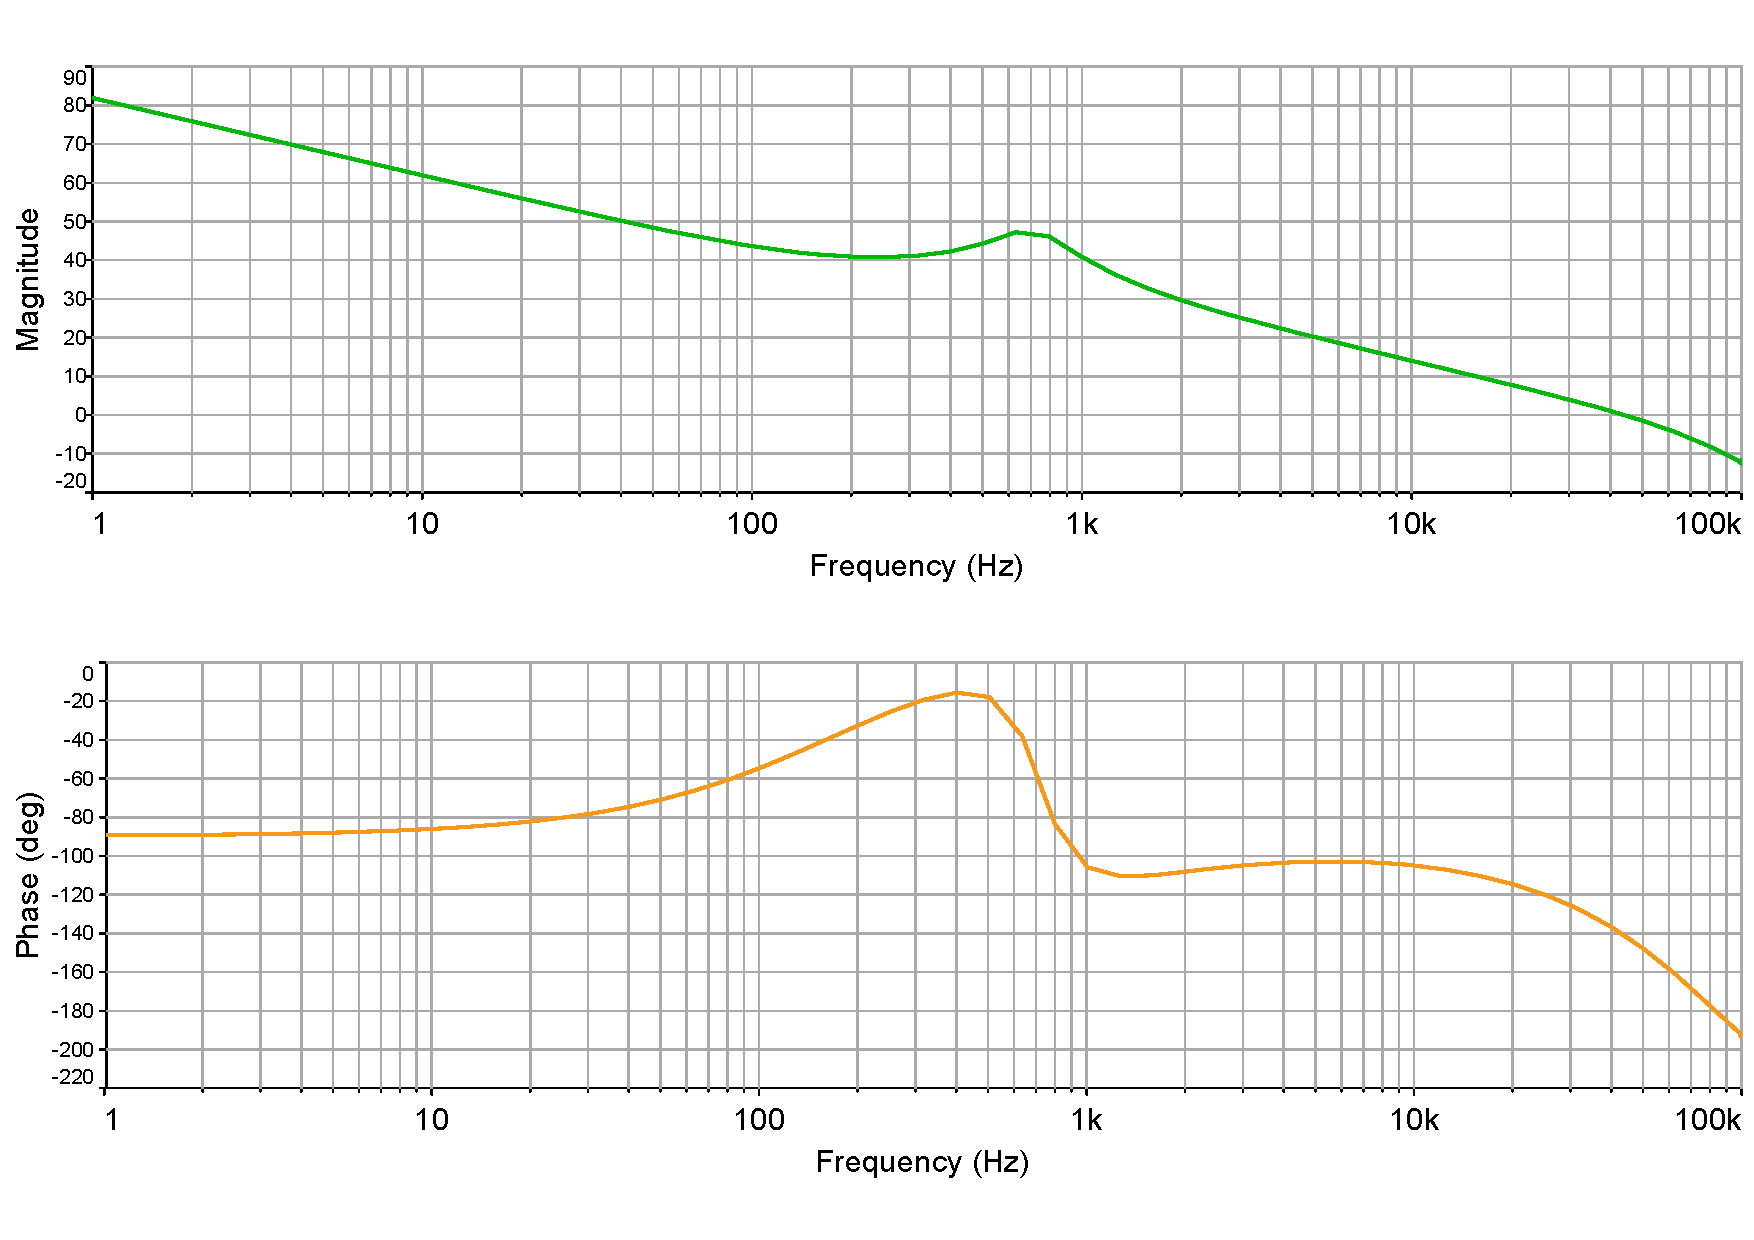
\includegraphics[width=12cm]{BodeGraph.pdf}
  \caption{被自动翻转的bode图}
  \label{rotatedBode}
\end{figure}

问题原因

同一幅图片,XeLaTeX~编译出现图片翻转,而~pdfLaTeX~编译,输出正常。
原因可能是出现在~XeLaTeX~编译过程中会将有些~pdf~文件自身多余的旋转命令编译出来。

问题解决方法

第一种方法(抄自刘海洋大牛的方案):
使用命令\\ \texttt{pdfcrop foo.pdf foo-new.pdf},当然,新文件名可以和旧文件名相同。 这个方法的好处就是 pdfcrop 是texlive自带的,我装的是texlive2017,因此自带了。

第二种方法:采用GhostScript软件消除多余的旋转命令。
\begin{enumerate}
    \item 下载安装~GhostScript~软件,官网为\url{https://www.ghostscript.com/download/gsdnld.html/}
        
    \item 将安装后的bin文件夹地址加入用户环境变量,在我电脑上为~\verb|D:|\verb|\Program Files|\verb|\gs|\verb|\gs9.22|\verb|\bin|
	
    \item cmd~命令行进入想转换图片所在文件夹,执行命令\\gswin32c -sDEVICE=pdfwrite -o newname.pdf  previousname.pdf
              得到一个去除多余旋转命令的~newname.pdf~文件。

    \item 在\LaTeX{}中插入该~pdf~文件,XeLaTeX~编译。
\end{enumerate}

处理之后的图片如图~\ref{Bode}~所示。
\begin{figure}[H] 
  \centering
  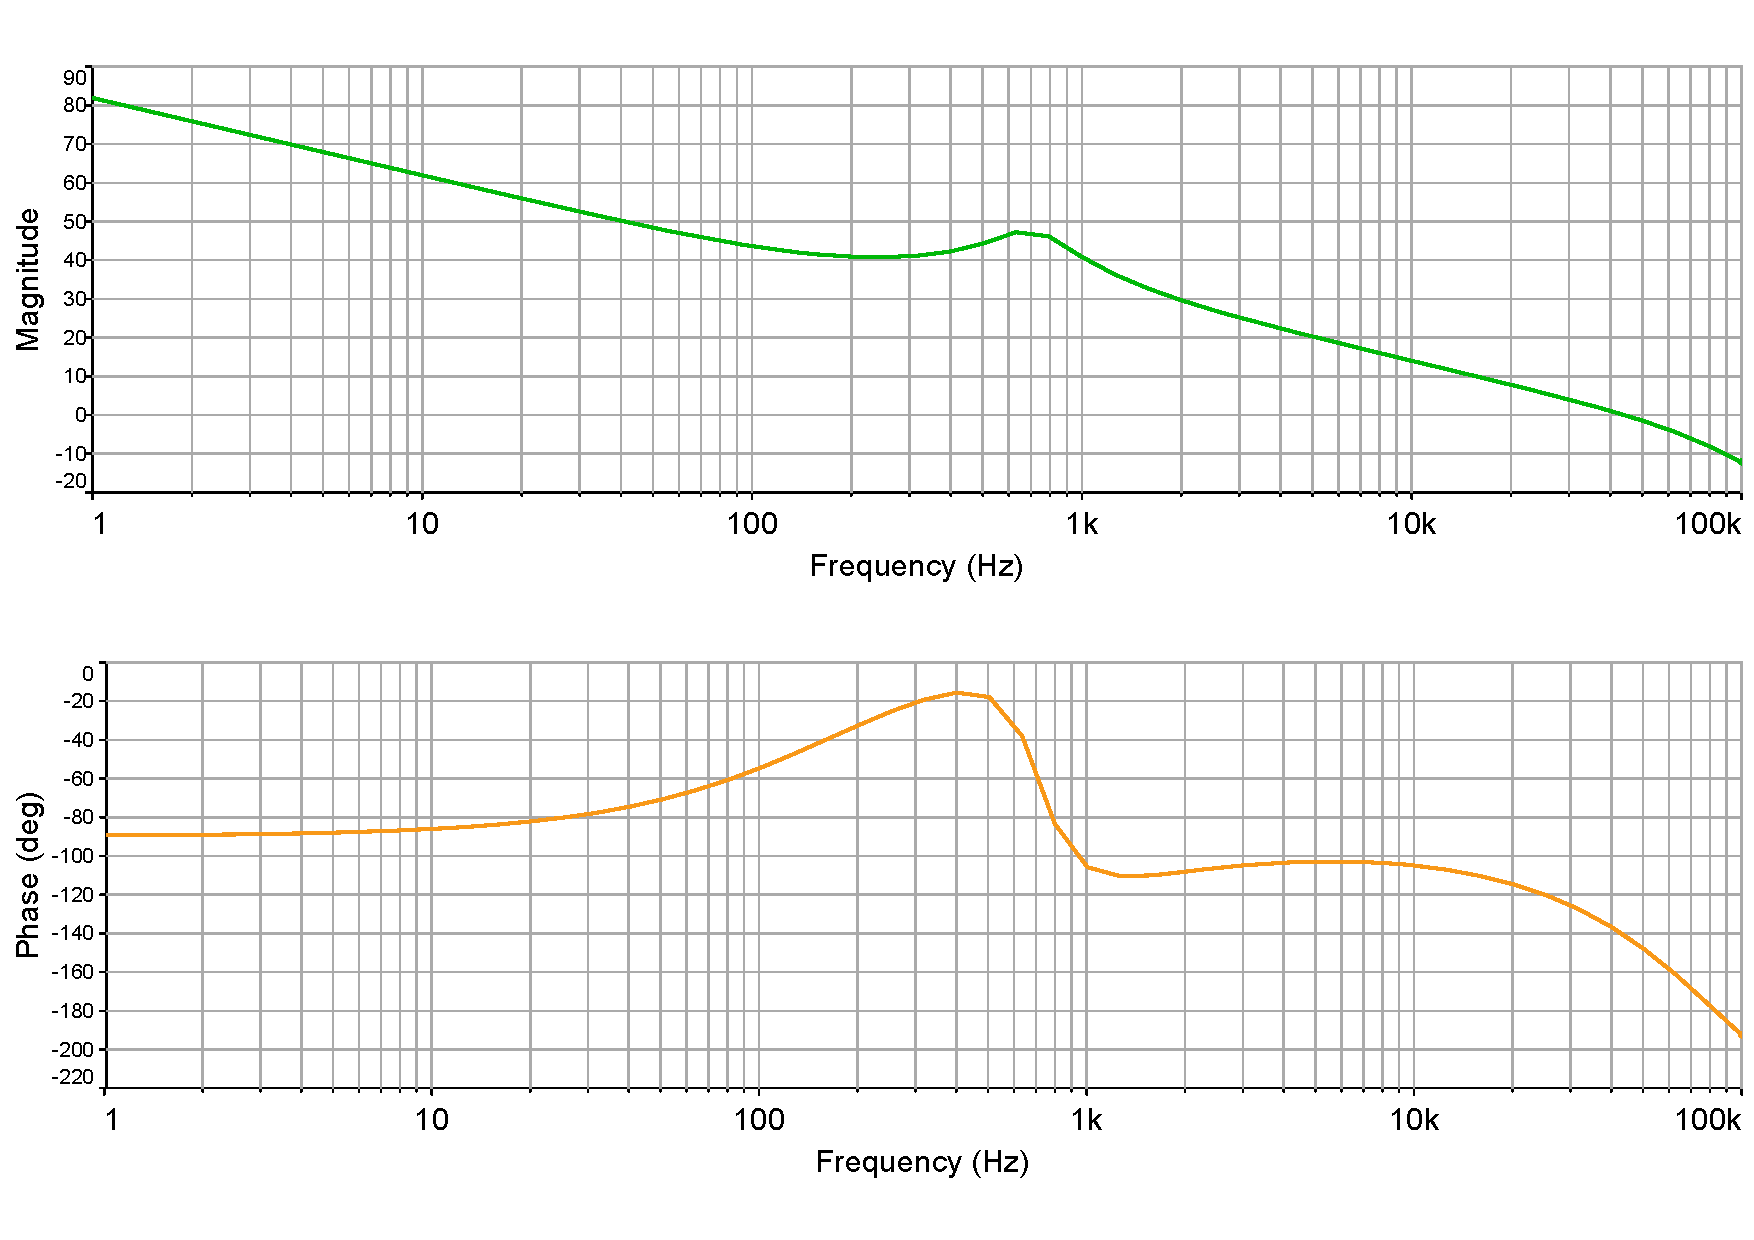
\includegraphics[width=12cm]{Bode.pdf}
  \caption{处理后的bode图}
  \label{Bode}
\end{figure}





